\documentclass[
  shortnames]{jss}

\usepackage[utf8]{inputenc}

\providecommand{\tightlist}{%
  \setlength{\itemsep}{0pt}\setlength{\parskip}{0pt}}

\author{
Shannon K. Gallagher\\Biostatistics Research Branch\\
National Institute of Allergy\\
and Infectious Diseases \And Benjamin LeRoy\\Dept. of Statistics \& Data Science\\
Carnegie Mellon University
}
\title{Time invariant analysis of epidemics with \pkg{EpiCompare}}

\Plainauthor{Shannon K. Gallagher, Benjamin LeRoy}
\Plaintitle{Time invariant analysis of epidemics with EpiCompare}
\Shorttitle{\pkg{EpiCompare}}

\Abstract{
We present \pkg{EpiCompare}, an \proglang{R} package that suppliments
and enhance current infectious disease modeling analysis pipelines as
well as to encourage comparisons across these pipelines. A major
contribution of this work is the set of novel \textit{time-invariate}
tools for model and epidemic comparisons - including time-invariate
prediction bands. \pkg{EpiCompare} encorporates \proglang{R}'s
\textit{tidy} coding style to aid it rapid and easy use. This paper
provides an overview of both the tools in and intuition behind
\pkg{EpiCompare} and a thorough demonstrating of the tools through a
detailed example of a full data analysis pipeline.
}

\Keywords{keywords, not capitalized, \proglang{Java}}
\Plainkeywords{keywords, not capitalized, Java}

%% publication information
%% \Volume{50}
%% \Issue{9}
%% \Month{June}
%% \Year{2012}
%% \Submitdate{}
%% \Acceptdate{2012-06-04}

\Address{
    Shannon K. Gallagher\\
    Biostatistics Research Branch\\
  National Institute of Allergy\\
  and Infectious Diseases\\
    5603 Fishers Lane\\
Rockville, MD 20852\\
  E-mail: \email{shannon.gallagher@nih.gov}\\
  URL: \url{http://skgallagher.github.io}\\~\\
      Benjamin LeRoy\\
    Dept. of Statistics \& Data Science\\
  Carnegie Mellon University\\
    5000 Forbes Ave.\\
Pittsburgh, PA 15213\\
  E-mail: \email{bpleroy@andrew.cmu.edu}\\
  URL: \url{https://benjaminleroy.github.io/}\\~\\
  }


% Pandoc header
\usepackage{booktabs}
\usepackage{longtable}
\usepackage{array}
\usepackage{multirow}
\usepackage{wrapfig}
\usepackage{float}
\usepackage{xcolor}

\usepackage{amsmath}

\begin{document}

\newcommand{\shannon}[1]{\textcolor{orange}{#1}}
\newcommand{\ben}[1]{\textcolor{violet}{#1}}

\newtheorem{theorem}{Theorem}

\section[Intro]{Introduction}\label{sec:intro}

The recent (and on-going) COVID-19 global pandemic has galvanized public
interest in understanding more about infectious disease modeling and has
highlighted the usefulness of research in the area of infectious disease
epidemiology. Infectious diseases inflict enormous burdens on the world:
millions of lives lost and trillions of dollars spent yearly. Infectious
disease models typically attempt to do one or more of the following: 1)
predict the spread of current and future epidemics
\citep[e.g. flu prediction][]{Biggerstaff2016}, 2) analyze past and
current epidemics to increase scientific knowledge
\citep[e.g. historical measle outbreaks][]{Neal2004}, and 3) forecast or
project epidemic scenarios under pre-specified parameters
\citep[e.g.][]{ferguson2020}. At the same time, descriptive statistics
and visualizations from universities, many branches and levels of
government, and news organizations are an important first step of the
process \citep{dong2020,cdc-covid-tracker2021,wp-covid-tracker2021} .

With the many visualization and exploratory tools, models and modeling
paradigms, and reviews and comparisons in the literature and through the
MIDAS (Models of Infectious Disease Agent Study) network
\citep{midasnetwork2021}, this field has a lot of devices to aid an
individual practitioner decide the correct approach. For
example,\proglang{R} packages such as \pkg{surveillance},
\pkg{EpiModel}, and \pkg{pomp} have all made significant steps in
standardizing the flow of the data analysis pipeline for epidemic
modeling through digitizing data sets, making accessible statistical
models, and providing a plethora of educational material for both coding
novices and experts alike \citep{surveillance2017,Jenness2018,King2016}.

At the same time, analysis packages often only address a specific
portion of the analysis pipeline, for instance focusing on certain types
of models. Modeling tools, which usually require learning
package-specific syntax, often don't provide easy ways to compare and
assess their models on new data. Moreover, exploring and modeling
epidemics require transforming and \textit{tidying} data in different
ways. To fill these gaps, we present our \proglang{R} package
\pkg{EpiCompare}. Our package's primary focus is to aid and advance
research in the area of comparison and assessment of epidemic and
epidemiological models. In Figure \ref{fig:pipeline}, we illustrate the
data analysis pipeline of infectious diseases as 1) data pre-processing,
2) exploratory data analysis (EDA), 3) modeling and simulating, 4)
post-processing, and 5) comparison and assessment; where each previous
part of the pipeline influences the next. \pkg{EpiCompare} provides
tools to aids practitioners in all areas of this pipeline.

\begin{figure}[!ht]
    \centering
    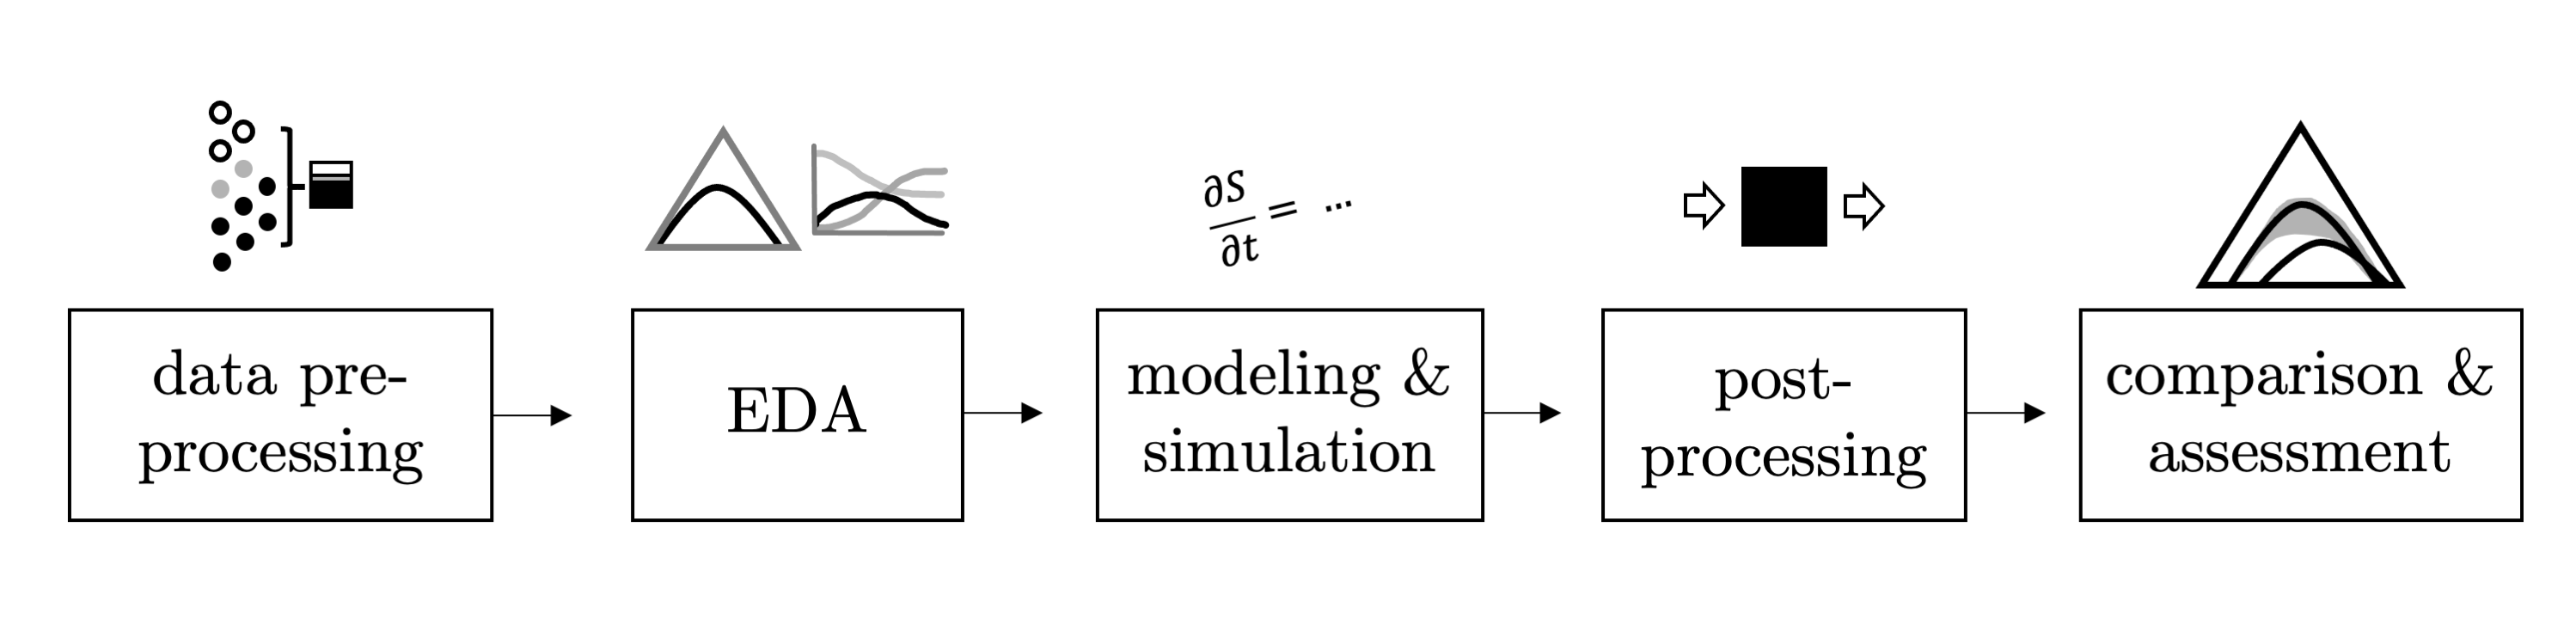
\includegraphics[width = 1\textwidth]{images/pipeline1.png}
    \caption{An idealized epidemiological data analysis pipeline.}
    \label{fig:pipeline}
\end{figure}

\pkg{EpiCompare} also emphasizes the value of analyzing epidemics in a
\textit{time-invariant} way. Epidemics, despite by definition being a
process that evolves over time, often need to be compared in a way not
constrained to initial times or time scales to understand the processes
at play. Additionally, many tools designed to examine the quantity of
the population in each epidemic state (for example: quantity of
Susceptible vs Infectious vs Recovered individuals) don't always as
intelligently capture the natural connections between the proportion of
individuals in these states.
\textcolor{orange}{I don't quite understand this.  Is this because of underreporting?  If so I'm not sure how EpiCompare helps us here.}
Tools in \pkg{EpiCompare} give the user the ability to extend their
toolkit to evaluate epidemics within a time-invariant lens. The goal of
\pkg{EpiCompare} is not to supplant existing infectious disease modeling
tools and software but, rather, is a concerted effort to create standard
and fair comparisons among models developed for disease outbreaks and
outbreak data.

This paper is broken up into the following sections, section
\ref{sec:time-invariant} motivates and showcases tools of time-invariant
analysis, section \ref{sec:overview} presents an outline of how
\pkg{EpiCompare} aids a practitioner in every step of the pipeline and
section \ref{sec:tour} provides a thorough demonstrating of the tools
through a detailed example of a full data analysis pipeline.

\section[Time-invariant]{Motivation and tools for time-invariant
analysis}\label{sec:time-invariant}

Epidemics can be difficult to compare to one another due to differences
in diseases, locations, or population behaviors, or times. In
\pkg{EpiCompare}, we emphasize comparisons between epidemics adjusting
for the last component, time. Time-invariant analysis is beneficial
because by adjusting for the unit of infection rate, we can focus on the
``lifetime'' of an epidemic, a view that is concerned more with the
number of lives affected than as opposed to any specific time
constraint. Time-invariant analysis is also beneficial when there are
gaps in time between occurrences of outbreaks of a similar nature in
different geographic regions. Finally, time-invariant analysis is
beneficial because many studies talk about a period of ``exponential
growth'\,' of the number of outbreaks
\citep{chowell2007,wallinga2007generation,forsberg2008}.

Time-invariant analysis, as it appears in \pkg{EpiCompare} solves the
above issues by observing functionals which attempt to capture the
general shape of the epidemic with respect to the proportion of the
population in each epidemic state. This allows us to compare scenarios
as different as, for instance as a decades-long outbreak HIV in the US
compared to a 10 day outbreak of norovirus on a cruise ship. Moreover,
this tool avoids the need for choosing a `beginning' \(t_0\) or `end'
\(t_F\) of an epidemic, choices \cite{gallagher2020} show that can
heavily influence, for example, estimates of peak infection height or
the reproduction number \(R_0\).

\subsection[r0]{\(R_0\) and time-invariant analysis}\label{r0}

By definition, \(R_0\) is the number of expected secondary infections
when a primary infection is introduced to a susceptible population.
\(R_0\) is also, maybe, the most famous \textit{time-invariant}
numerical summary of an epidemic, which allows epidemics to be compared
to one another in both different time and geographic scales. For
example, \(R_0\) for Covid-19 is estimated to be between 2-3, seasonal
influenza between 1.2-2, and modern measles outbreaks between 5-6
\citep{midas2020,biggerstaff2014,namee2018}.

Estimator(s) for \(R_0\) are dependent on the epidemic modeling
framework, which consists of which states an individual can occupy
(e.g.~susceptible, infectious, recovered) and a description of how
individuals move from one state to the next over time (see
\cite{hethcote1994}). A common epidemic modeling framework is the SIR
model, originally introduced by \citet{kermack1927}. Transitions from
one state to the next are defined by a series of ordinary differential
equations, where \(N\) is the (fixed) total number individuals,
\(\beta\) is the rate of infection, and \(\gamma\) is rate of recovery,
\begin{align}\label{eq:sir-ode}
      S^\prime(t) &= -\frac{\beta S(t)I(t)}{N} \\
      I^\prime(t) &= \frac{\beta S(t)I(t)}{N} - \gamma I(t) \nonumber\\
      R^\prime(t) &= \gamma I(t) \nonumber.
  \end{align} From this,
\(\hat{R}_0 = \frac{\hat{\beta}}{\hat{\gamma}}\), the ratio of the
estimated infection rate compared to the estimated recovery rate.

With regards to traditional epidemic \(state\) vs.~\(time\) plots,
\(R_0\) is difficult to visualize, especially with respect from one
epidemic to another. For example, consider the scenarios where the first
epidemic is generated from a SIR model with \((S(0) = 990, I(0) = 10)\),
\(\beta_1 = 0.3\) and \(\gamma_1 = 0.15\), and the second epidemic is
generated from a SIR model with \((S(0) = 990, I(0) = 10)\),
\(\beta_2 = 0.24\) and \(\gamma_1 = 0.12\) over 40 days. Both epidemics
have the same value of
\(R_0 = \beta_1/ \gamma_1 = \beta_2 / \gamma_2 = 2\). The epidemic
trajectories are shown in the \(state\) vs.~time plots in Figure
\ref{fig:sir-ex}. At a glance, we may assume that Model 1 has a larger
\(R_0\) than Model 2 because the peak of infection occurs more quickly
than in Model 2. On the other hand, we may think Model 2 has a larger
\(R_0\) because it has a slightly larger peak of infection than Model 1.

\begin{CodeChunk}
\begin{figure}[H]

{\centering 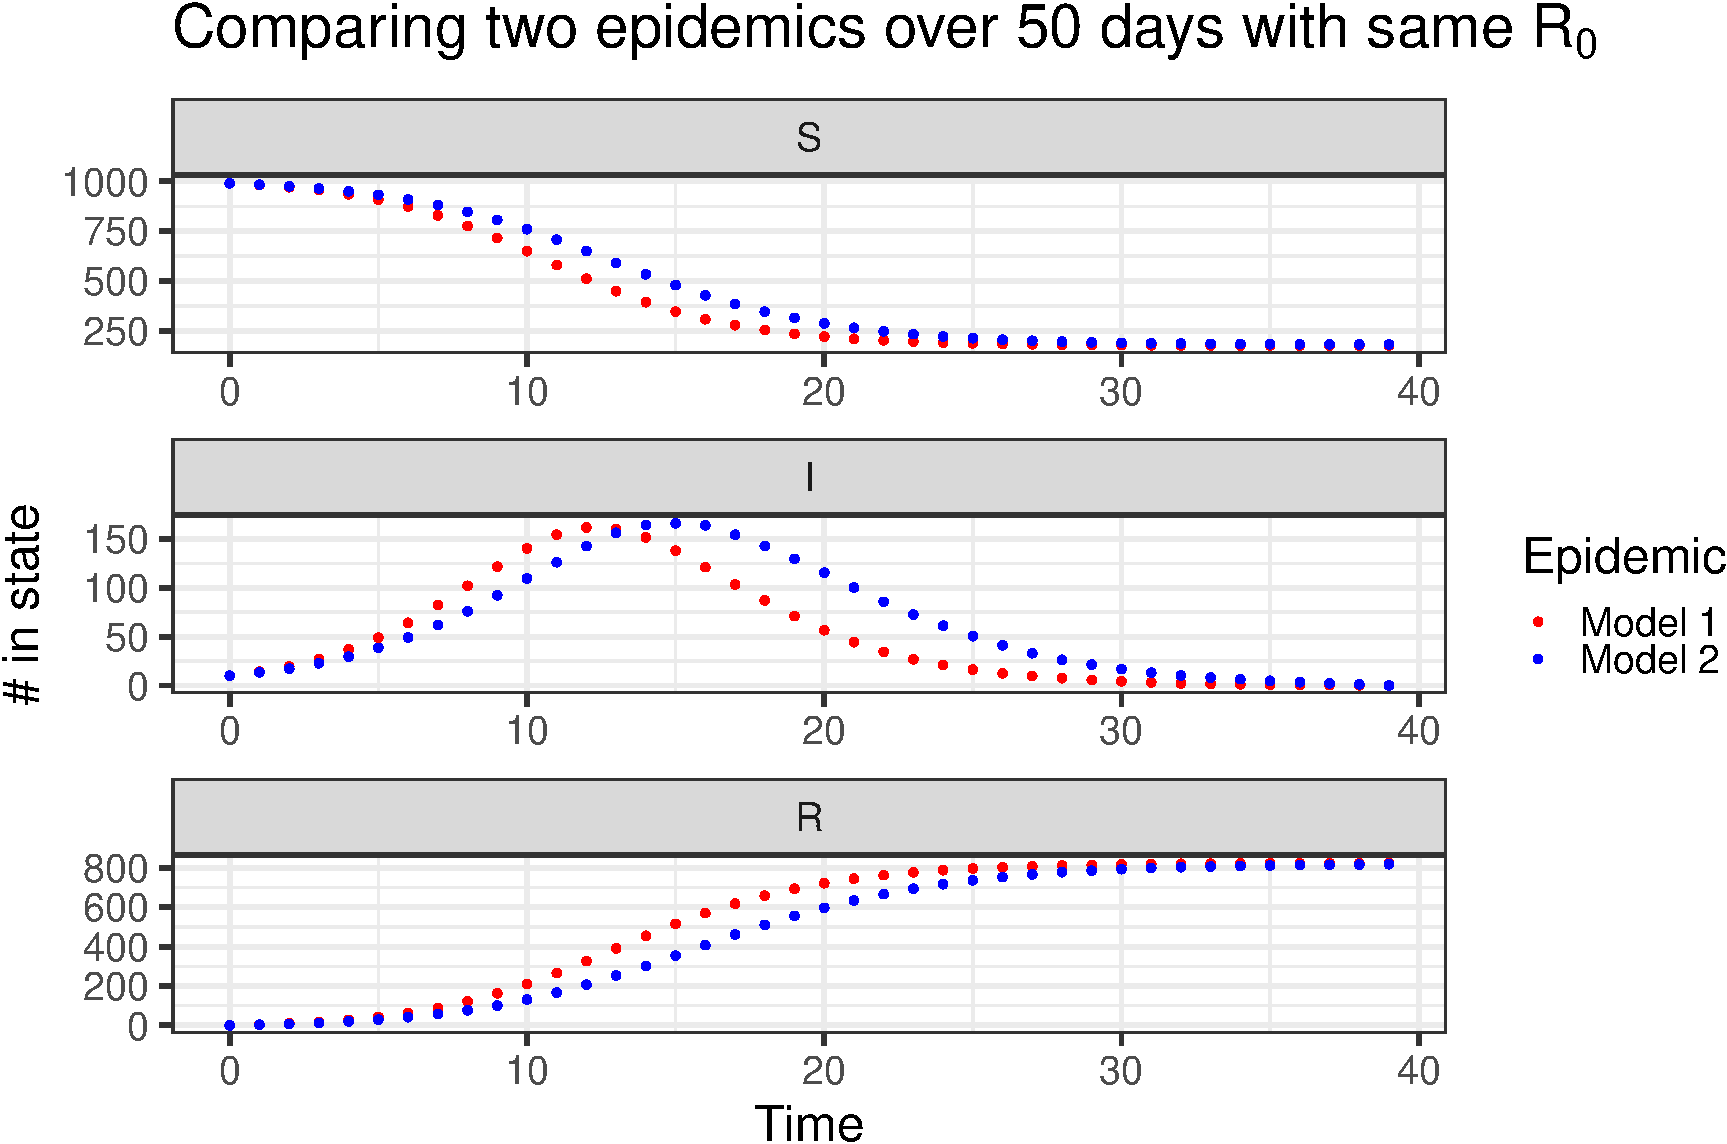
\includegraphics{Figs/unnamed-chunk-2-1} 

}

\caption{\label{fig:different-scales-standard}Example of two epidemics with different $\beta$ and $\gamma$ paremeters but the same initial reproduction number $R_0$ = 2.  Both plots are generated from models with $N= 1000$ individuals with $S(0) = 990$ and $I(0) = 10$.}\label{fig:unnamed-chunk-2}
\end{figure}
\end{CodeChunk}

However, when we plot the trajectories as a single curve using the
ternary plot in the time-invariant view, we immediately see a different
story. In this time-invariant view in Fig. \ref{fig:ternary-ex}, the
points seem to overlap and form the same trajectory. In other words, we
can see there is something fundamentally linking these two different
epidemics, and this fundamental link turns out to be \(R_0\).

More formally, let two Kermack and McKendrick (see Eq.
\eqref{eq:sir-ode}) SIR models be denoted \((S_1(t), I_1(t), R_1(t))\)
and \((S_2(t), I_2(t), R_2(t))\), respectively, for \(t > 0\). Assume
both models have initial values \((S(0), I(0), R(0))\). Let
\(R_0 = \frac{\beta_1}{\gamma_1} = \frac{\beta_2}{\gamma_2}\) where
\(\beta_i\) and \(\gamma_i\) are the average infection rate and recovery
rate, respectively, for SIR model \(i=1, 2\). Equivalently,
\(\beta_2 = a \beta_1\) if and only if \(\gamma_2 = a \gamma_1\) for
some \(a > 0\).

\begin{theorem}\label{thm:sir-scale}
Let there be two SIR models as described above.  Then for all $t > 0$ there exists an $s$ such that $(S_1(t), I_1(t), R_1(t)) = (S_2(s), I_2(s), R_2(s))$.  Moreover, $s = \frac{1}{a}t$.
\end{theorem}

The proof of Theorem \ref{thm:sir-scale} relies on a fairly recent
result from \cite{Harko2014} and is shown in detail in Appendix
\ref{app:proof}. The consequence of Theorem \ref{thm:sir-scale} is that
for two SIR models that have the same initial percent of individuals in
each state and \(R_0\) then for every point on the epidemic path of the
first SIR model is also a point on the epidemic path of the second SIR
model. Taking the sample simulations from Fig.
\ref{fig:different-scales-standard}, Fig.
\ref{fig:different-scales-tern} presents these two models in a ternary
plot. This means with our time-invariant ternary plot, that at a glance,
we can tell if two epidemics have different values of \(R_0\).

\begin{CodeChunk}
\begin{figure}[H]

{\centering 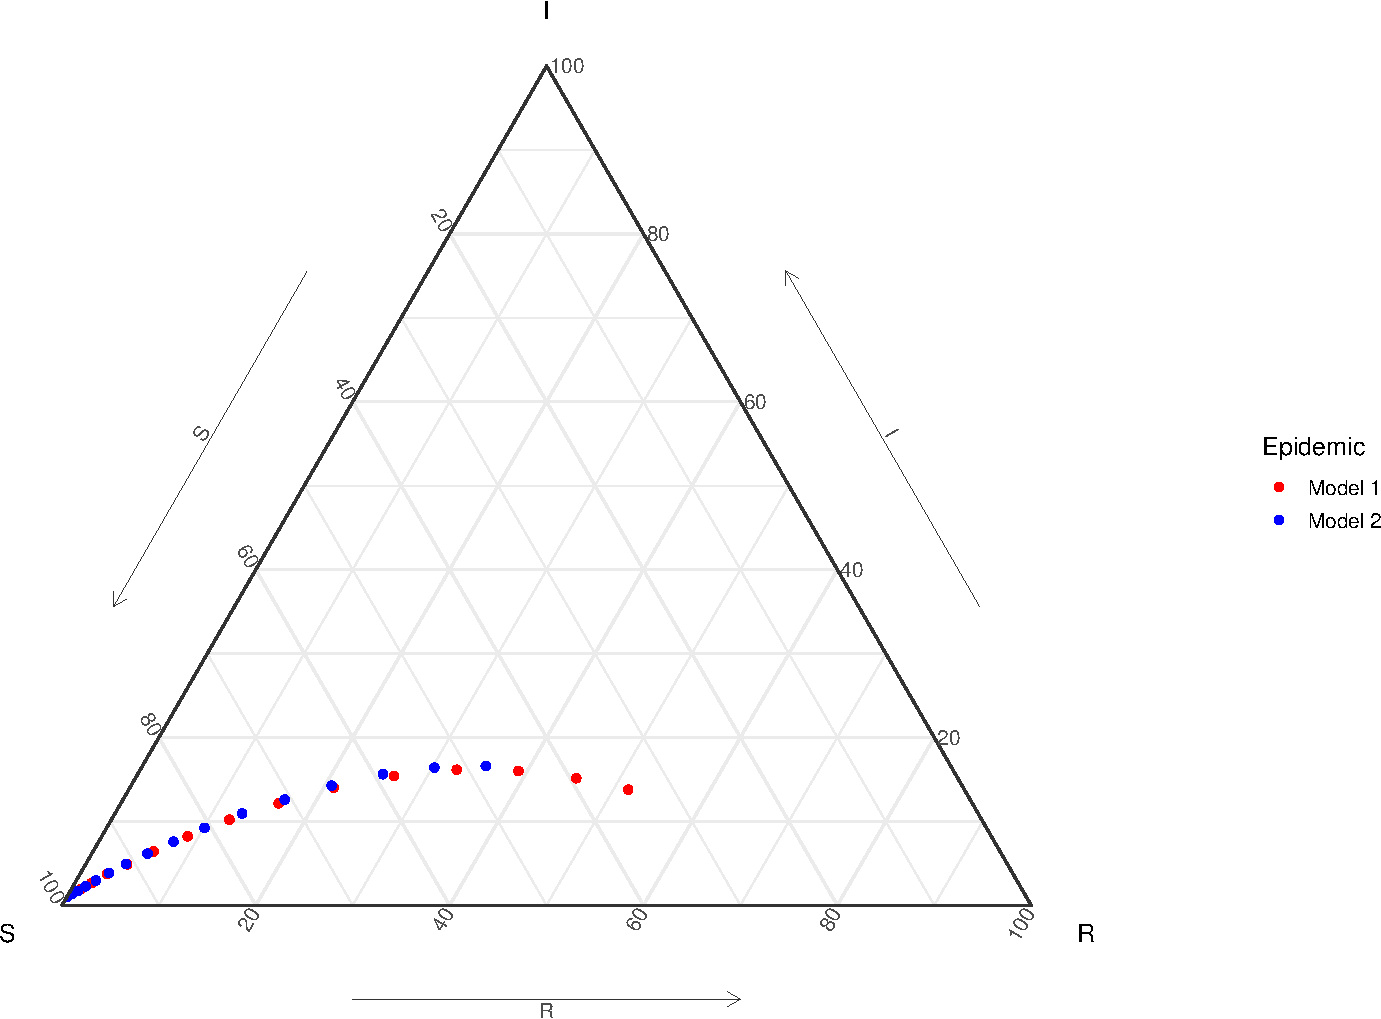
\includegraphics{Figs/unnamed-chunk-3-1} 

}

\caption{\label{fig:different-scales-tern}Example of two epidemics with different $\beta$ and $\gamma$ paremeters but the same initial reproduction number $R_0$ = 2.  Both plots are generated from models with $N= 1000$ individuals with $S(0) = 990$ and $I(0) = 10$.  These are plotted in the time-invariant view, where we can see the number of susceptible, infectious, and recovered.}\label{fig:unnamed-chunk-3}
\end{figure}
\end{CodeChunk}

\hypertarget{beyond-the-kermack-and-mckendrick-sir-models}{%
\subsection{Beyond the Kermack and McKendrick SIR
models}\label{beyond-the-kermack-and-mckendrick-sir-models}}

Although the result of Theorem \ref{thm:sir-scale} allows for easy
visual comparison of \(R_0\) in Kermack SIR models, it does require
stringent assumptions of homogeneity of behavior in populations. The use
of visualizing epidemics in a time-invariant lens via ternary plots
extends beyond those of models that follow the ODEs in the
Kermack-McKendrick equations. Any model with S, I, and R states can be
visualized with ternary plots, regardless of birth and death dynamics
and regardless of homogeneity of individual behavior. We can use ternary
plots to compare the spread of a disease for groups within a population
without time as a confounding factor. We show an example of this in a
later section.

But time-invariant analysis is also useful for epidemic models with more
than three states. The constraints in three dimensions that are met with
the SIR model (that is
\(\sum_{i=1}^3 (\text{number in state}(i)) = N(t)\)) actually represents
a space of 3d simplices, and the ternary plot specifically represents
these simplices, after scaling to examine such values as proportions
between 0 and 1 (ternary plots are known as a 3d unit simplex due to
it's scaling). This same scaling for larger models (i.e.~with more
states) can be done onto different simplexes. In this package we present
tools to help compare models (mostly through simulations). s tool
compares these objects after projecting them into a one-dimension-fewer
space through the simplexical structure of the data.

In \pkg{EpiCompare} we allow for the comparison epidemics in these
higher dimensional spaces by first projecting onto these simplexes. Even
though higher dimensional models may not be able to visualized, we
provide multiple tools to aid in the comparison of models and epidemics.
The first of which uses multiple simulations under specific model
parameters to assess the bairabilty of the model fit. In
\pkg{EpiCompare} we provide ways to create prediction regions for a true
epidemic under the model assumptions using these simulations. These
regions require representing multi-dimensional structures for functions
to completely contain epidemics, and treat these simulations and
epidmeics as filamental objects. We extend off of papers like
\citet{Dalmasso2019a} to create these bands. These high dimensional
bands allow the user to assess if the true epidemic is within the band
(there-by assessing the model's representation of the epidemic), and
also compare who different models are from each other through distances
that compare sets. We recommend using the Hausdorff distance to compare
such sets as it captures how much bigger the sets would have to expand
to cover each other, and is defined mathematically as \[
d_\text{Hausdorff}(S_1, S_2) = \max \left\{ \sup_{x \in S_1} \inf_{y \in S_2} d(x,y) \;,\; \sup_{y \in S_2} \inf_{x \in S_1} d(x,y)\right\}\;.
\]

\section[Package overview]{Package tool overview}\label{sec:overview}

\textcolor{violet}{**The goals of this section is to present parts of the data science pipeline, introduce how we help, why they are useful and the ideas behind it.**}

In this section we will present the tools in this package and how they
aid in the data analysis pipeline. We present a modification of Figure
\ref{fig:pipeline} from the Section \ref{sec:intro} with Figure
\ref{fig:pipeline2} with uses of our package. We recommend the package
user keep this image around as a reference. All user functions are aimed
to be as friendly as possible, and we focus on providing the user
``tidyverse'' style functions, that encourage piping and also follow
clear verb naming schemes \citep{Wickham2019}. There are 2 different
ways \pkg{EpiCompare} can be incorporated in the data analysis pipeline
for epidemics, either at the very beginning when pre-processing data and
visualizing raw data, or after modeling has been done and a generative
model is fit. Figure \ref{fig:pipeline2} captures these different paths,
and we will highlight both approaches and how to leverage
\pkg{EpiCompare} in the subsections below.

\begin{figure}[!ht]
    \centering
    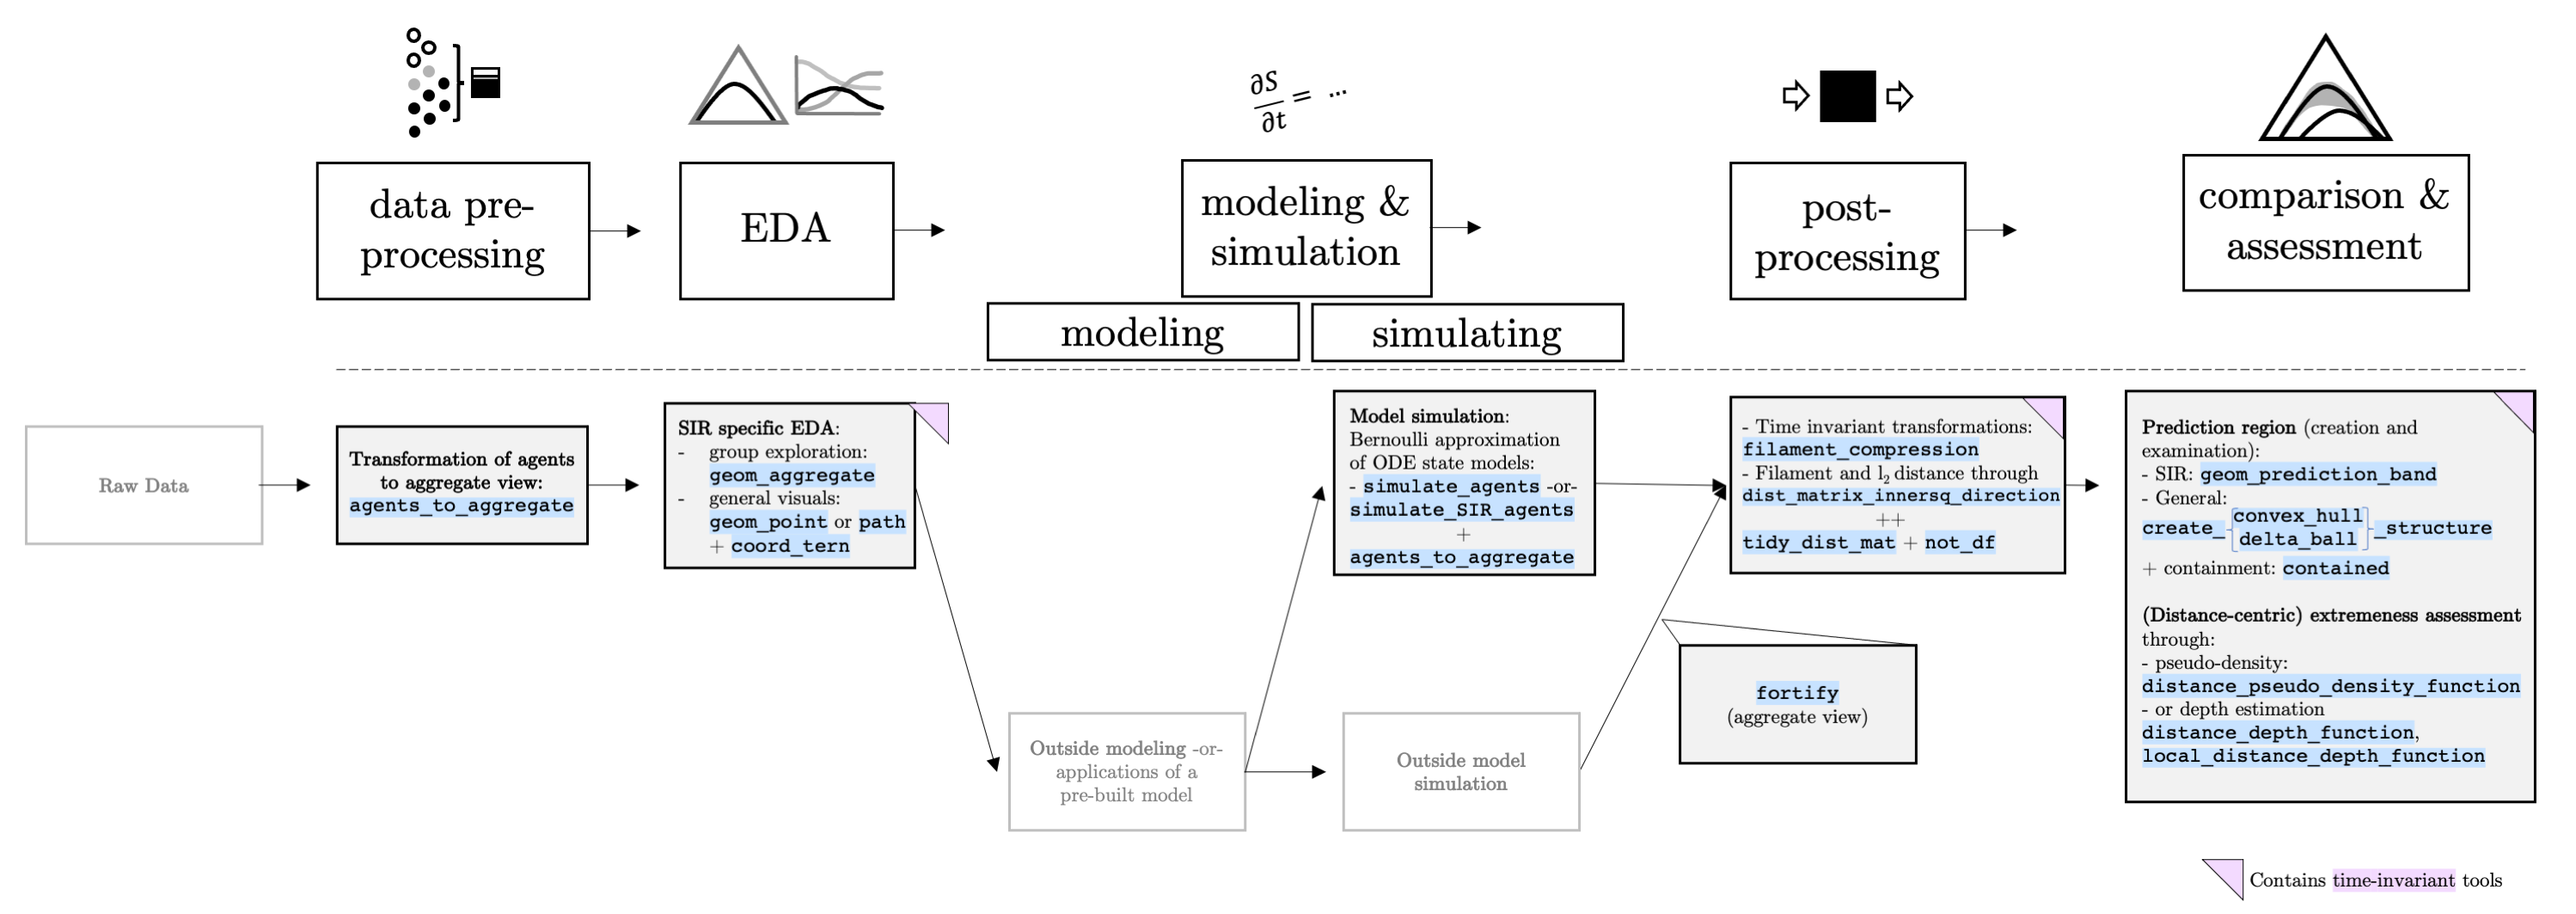
\includegraphics[width = 1\textwidth]{images/pipeline2.png}
    \caption{How \pkg{EpiCompare} supplements and aids in the epidemiological data analysis pipeline.}
    \label{fig:pipeline2}
\end{figure}

\hypertarget{data-preprocessing}{%
\subsection{Data Preprocessing}\label{data-preprocessing}}

The first step of most data analysis is cleaning up the data to be
explored. There are multiple ways to collect the epidemiological data.
Sometimes individual records with times of different states of the
epidemic (infection, recovery, etc.) as well as individual information
like network structure, location, and-sub population information will be
collected, whereas other data collections will focus
population/sub-population counts of individuals in each epidemic
state\footnote{\@Shannon include citations}. We focus on understanding
the overall impact on the population/sub-populations we provide a
function to transform information about each agent's start time of each
state (e.g.~start of infection, etc). This transformation between from
agent information to aggregate information is very useful for seeing the
overall trend of the epidemic (and how it impacts different
subpopulations). Our tools aim to allow the user to easily group agents
and define new subpopulations to explore. This is important as many case
studies have highlighted the usefulness to identify differing
subpopulations\footnote{\@Shannon cite} and many state based models
provide for subpopulation based states in their
analysis\footnote{\@Shannon cite}.

We provide a ``tidyverse''-styled function,
\texttt{agents\_to\_aggregate} to transform agent information into
aggregate state information, As a ``tidy'' function, our function
\texttt{agents\_to\_aggregate} allows the user to identify any
subpopulations by first doing \texttt{group\_by} from \texttt{dplyr},
and also allows for infinite epidemic states - which can be for models
with assumptions of sub population based states (e.g.~youth infections),
as well as indicators for death and birth dates. Our function,
\texttt{agents\_to\_aggregate} allows for states to be skipped -
captured with \texttt{NA} values and multiple starts of a state -
(e.g.~multiple infections) as long as the original data is stored in
columns that are constrained to ordering
ideas\footnote{make this more clear?}. Currently this function is
constrained to integer time steps (for example days), but
transformations (linear or otherwise) of the time columns can make the
time steps more (or less) . \texttt{agents\_to\_aggregate} then returns
a standardized count for each state for each time point. We see
\texttt{agents\_to\_aggregate} as a really powerful tool, but also very
useful to quickly transform agents information to be used in aggregate
state-based models and compare state-based models to observed data.

\hypertarget{eda}{%
\subsection{EDA}\label{eda}}

With raw data, getting to know our data now-a-days very frequently means
figuring out good combinations of visualizations, numerical summaries
and subsetting. An expert coder can start from
\texttt{agents\_to\_aggregate} to successfully do this in many ways, but
we've also developed tools to rapidly explore your data if your have a 3
unique states models (like the SIR model). Our \texttt{geom\_aggregate}
provides a rapid way to explore different subpopulations experience of
the epidemic, and combines the ideas behind agents\_to\_aggregate for
the SIR case, with \texttt{geom\_path} and \texttt{coord\_term} to
visualize any number of groups epidemic trajectory in 3d simplex space
using \texttt{ggplot2} and \texttt{ggtern}
\citep{Wickham2016, Hamilton2018}. Visualization tools for SIR models
were developed because (1) SIR models are the most common and basic
state-based models\footnote{\@Shannon: cite} and (2) our simplex
representation of these epidemics emphasizes a ``time-invarance''
representation of the data (for a refresher see Section
\ref{sec:time-invariant}).

\hypertarget{model-fitting-and-simulations}{%
\subsection{Model Fitting and
Simulations}\label{model-fitting-and-simulations}}

Although this package does not focus on estimating a model for the data,
we do provide some power functions for simulation of basic state models
with Bernoulli approximation of ODE state models encoded in
simulate\_agents and simulate\_SIR\_agents (which can naturally be
combined with agents\_to\_aggregate ). \textbf{Description of these
models, reference to Shannon R0 paper, etc\ldots{}}

\hypertarget{post-processing}{%
\subsection{Post-processing}\label{post-processing}}

\ldots{}

\hypertarget{comparions-and-assessment}{%
\subsection{Comparions and Assessment}\label{comparions-and-assessment}}

\ldots{}

\section[Tour]{A tour of \pkg{EpiCompare}}\label{sec:tour}

In this section, we highlight a number of the functionalities available
in \kg{EpiCompare}. These functionalities include data cleaning,
visualization, simulation, and comparison, in accordance with the data
analysis pipeline \ref{fig:pipeline}. We show a full data analysis from
beginning to end that can be accomplished in a streamlined and
standardized manner.

\subsection{Data and exploratory analysis}

We analyze an outbreak of measles in the town of Hagelloch, Germany from
1861-1862, a data set organized by \cite{pfeilsticker1863}. The data was
later made visible by \cite{oesterle1992} and made available in an
\proglang{R} by \cite{surveillance2017}. The Hagelloch data includes a
rich set of features including household members, school level,
household locations, date of first symptoms (prodromes), date of measles
rash, and even the alleged infector. A subset of the data is shown in
Table \ref{tab:hags-people}. Because of these rich features, this data
set has been an ideal testing ground methodology in infectious disease
epidemiology and is used in work by
\cite{Neal2004,britton2011,groendyke2012,becker2016}.

\begin{CodeChunk}
\begin{table}[!h]

\caption{\label{tab:hags-people}Subset of Hagelloch infection data.  Features include the person ID, household ID (HH ID), age, sex, class level (Pre-K/1st/2nd), date of first symptoms, date of the appearance of the measles rash, and the alleged infector ID of the individual.}
\centering
\begin{tabular}[t]{rrlrllllr}
\toprule
ID & HH ID & Name & Age & Sex & Class & Symp. Start & Rash Date & Infector ID\\
\midrule
1 & 61 & Mueller & 7 & female & 1st class & 1861-11-21 & 1861-11-25 & 45\\
2 & 61 & Mueller & 6 & female & 1st class & 1861-11-23 & 1861-11-27 & 45\\
3 & 61 & Mueller & 4 & female & preschool & 1861-11-28 & 1861-12-02 & 172\\
4 & 62 & Seibold & 13 & male & 2nd class & 1861-11-27 & 1861-11-28 & 180\\
5 & 63 & Motzer & 8 & female & 1st class & 1861-11-22 & 1861-11-27 & 45\\
45 & 51 & Goehring & 7 & male & 1st class & 1861-11-11 & 1861-11-13 & 184\\
\bottomrule
\end{tabular}
\end{table}

\end{CodeChunk}

With \pkg{EpiCompare}, we can easily obtain the empirical cumulative
incidence function with respect to the measles rash appearance (variable
\code{ERU}) with the following tidy-style function,
\code{agents_to_aggregate}. The function \code{agents_to_aggregate} is a
key component of \pkg{EpiCompare}, allowing the user to easily switch
from an individual-level (i.e.~an agent) view of a disease to an
aggregate level. For example, the below code shows how we can convert
the agent data to a cumulative incidence of the measles rash, in order
to see how the disease spread through the population over time. We can
then compare the cumulative incidence of the rash to the cumulative
incidence of the prodromes, i.e.~the initial symptoms. We do this with
the below code, and a part of the cumulative incidence data output are
shown in Table \ref{tab:cif-rash}. The argument
\code{integer_time_expansion} indicates whether we should include all
time points in the recorded range of the data or only when there is a
change in the incidence.

\begin{CodeChunk}
\begin{CodeInput}
R> cif_rash  <- hagelloch_raw %>%
+   mutate(time_of_rash = as.numeric(ERU - min(PRO, na.rm = TRUE))) %>%
+   agents_to_aggregate(states = time_of_rash,
+                       integer_time_expansion = FALSE) %>%
+   mutate(type = "Rash")
\end{CodeInput}
\end{CodeChunk}

\begin{CodeChunk}
\begin{table}[!h]

\caption{\label{tab:cif-rash}Turning the individual-level information from the Hagelloch data to an aggregate view of the cumulative incidence of the measles rash in the population over time.}
\centering
\begin{tabular}[t]{rrr}
\toprule
Time & \# Susceptible & \# Total rash appearances\\
\midrule
0 & 188 & 0\\
4 & 187 & 1\\
7 & 186 & 2\\
9 & 185 & 3\\
12 & 183 & 5\\
\bottomrule
\end{tabular}
\end{table}

\end{CodeChunk}

One question of interest is the duration between initial onset of
prodromes or symptoms and the appearance of the measles rash. Since
\code{agent_to_aggregate} outputs a tidy-style data frame, it is a
simple task to plot the two sets of incidence curves on the same graph
(Fig. \ref{fig:cifs}).

\begin{CodeChunk}
\begin{CodeInput}
R> cif_prodromes <- hagelloch_raw %>%
+   mutate(time_of_PRO = as.numeric(PRO - min(PRO, na.rm = TRUE))) %>%
+   agents_to_aggregate(states = time_of_PRO,
+                       integer_time_expansion = FALSE) %>%
+   mutate(type = "Pro")
\end{CodeInput}
\end{CodeChunk}

\begin{CodeChunk}
\begin{CodeInput}
R> plot_df <- bind_rows(cif_rash, cif_prodromes)
R> 
R> ggplot(data = plot_df,
+        aes(x = t, y = X1, col = type)) + 
+   geom_step() + 
+   labs(title = "Cumulative incidence of measles appearance",
+        x = "Time (days relative to first prodrome appearance)",
+        y = "Cumulative incidence of event") + 
+   coord_cartesian(xlim = c(0, 55)) +
+   scale_color_manual(values = c("blue", "red"))
\end{CodeInput}
\begin{figure}[H]

{\centering 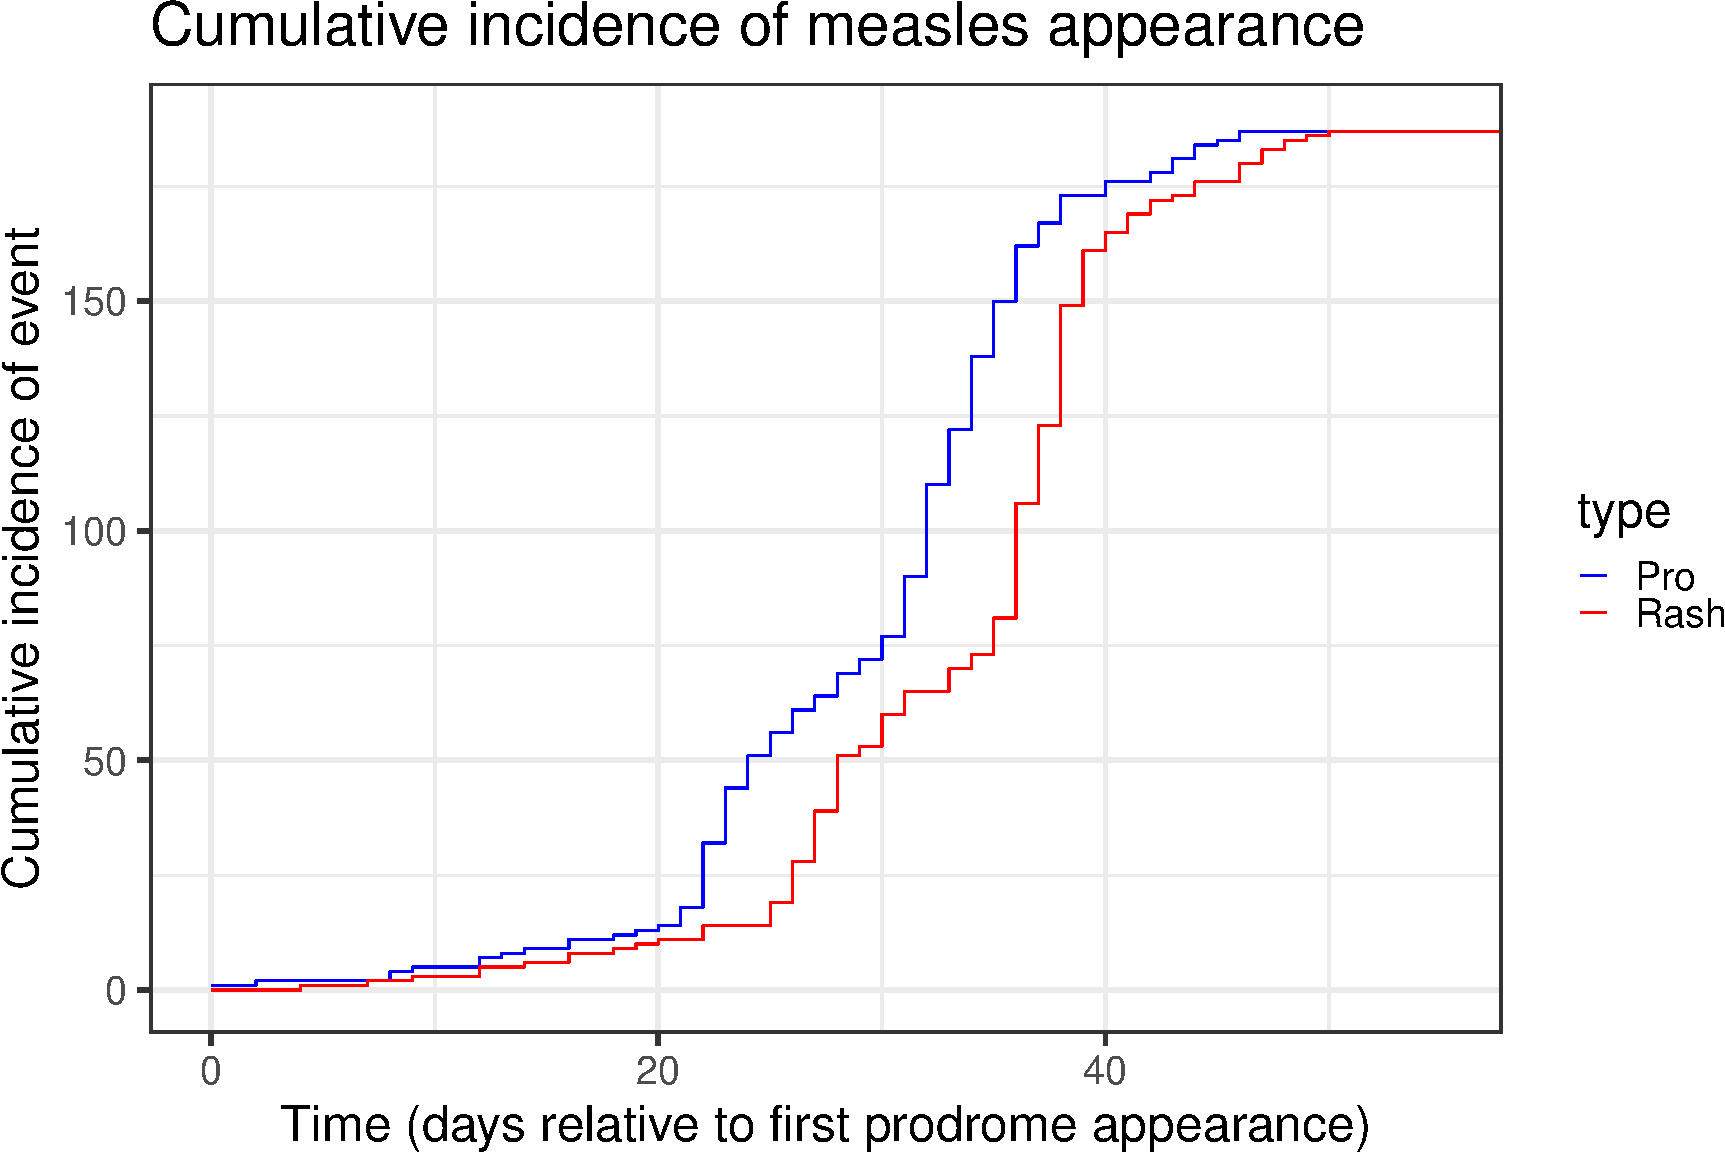
\includegraphics{Figs/unnamed-chunk-7-1} 

}

\caption{\label{fig:cifs}Empirical cumulative incidence functions of prodrome (symptom) onset and measles rash appearance.  We see that there is approximately a a constant lag between the two curves.}\label{fig:unnamed-chunk-7}
\end{figure}
\end{CodeChunk}

The real power of \code{agents_to_aggregate()} lies in its ability to
aggregate over any number of pre-specified states. For example, the
Hagelloch data sets contains two columns, \code{tI} and \code{tR}, the
time of infection and recovery, respectively of each individual. We can
then plot the SIR values through a time-invariant lens using
\pkg{ggplot2} and \pkg{ggtern} functions (as shown in Fig.
\ref{fig:hag-tern-raw}) or with our custom \code{geom},
\code{geom_aggregate}, which takes the raw agent data as input.

\begin{CodeChunk}
\begin{CodeInput}
R> hagelloch_sir <- hagelloch_raw %>%
+   agents_to_aggregate(states = c(tI, tR),
+                       min_max_time = c(0, 55)) %>%
+   rename(time = t, S = X0, I = X1, R = X2)
R> 
R> 
R> ggplot(hagelloch_sir, aes(x = S, y = I, z = R))+
+   coord_tern() +
+   geom_path() +
+   labs(x = "S", y = "I", z = "R",
+        title = "Time invariant view of Hagelloch measles outbreak") + 
+   theme_sir(base_size = 24)
\end{CodeInput}
\begin{figure}[H]

{\centering 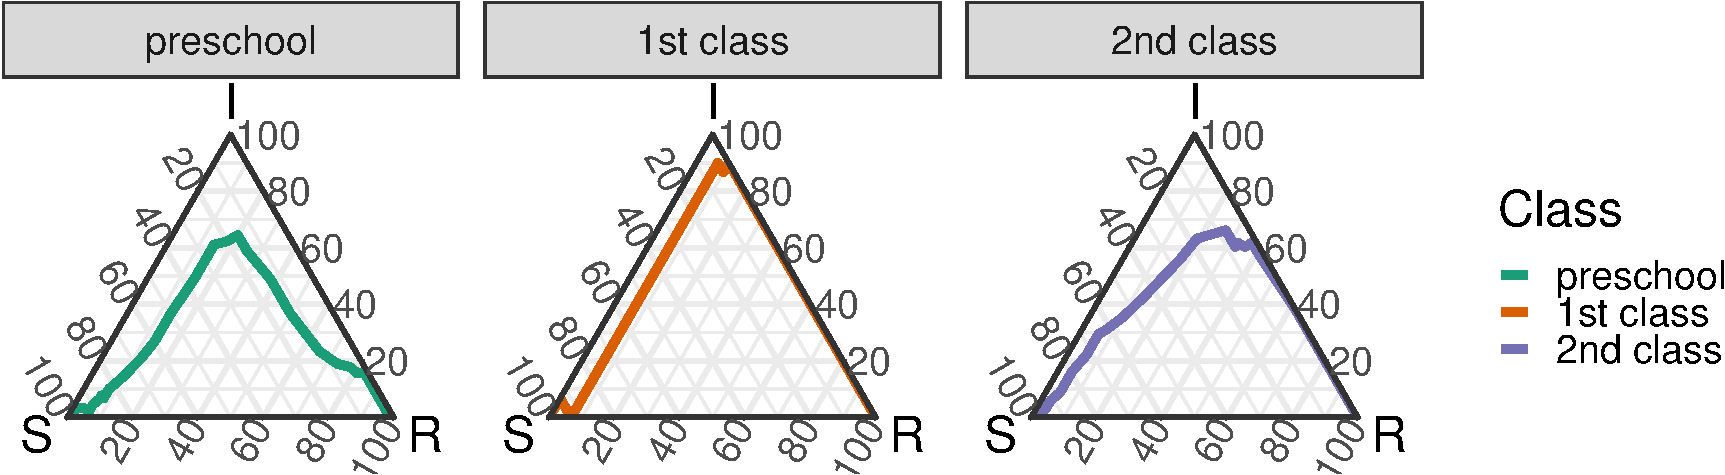
\includegraphics{Figs/unnamed-chunk-9-1} 

}

\caption{\label{fig:hag-tern-raw}Time invariant view of the Hagelloch epidemic where we view the individuals in Susceptible, Infectious, or Recovered states.  We see there are two peaks of infection (the vertical axis).}\label{fig:unnamed-chunk-9}
\end{figure}
\end{CodeChunk}

Moreover, we can look at the outbreaks of the disease by group within
\code{agent_to_aggregate()} or \code{geom_aggregate()}. This allows us
to examine differences among the different groups of individuals. For
example, we show the time invariant outbreak by class level in Figure
\ref{fig:tern-class-data}. Immediately, we see that time invariant
infection curve is different for the pre-school class compared to the
1st class. In the 1st class, we see about 95\% of the class become
infected and less than 10\% of them having recovered, which is
indicative of a super-spreading event. This suspicion is further
confirmed in that 26 of the 30 1st class students have been reportedly
infected by the same individual.

\begin{CodeChunk}
\begin{CodeInput}
R> hagelloch_raw %>%
+   ggplot(aes(y = tI, z = tR, color = CL)) +
+   geom_aggregate(size = 2) + coord_tern() +
+   labs(x = "S", y = "I", z = "R",
+        color = "Class") +
+   scale_color_brewer(palette = "Dark2") +
+   facet_wrap(~CL)
\end{CodeInput}
\begin{figure}[H]

{\centering 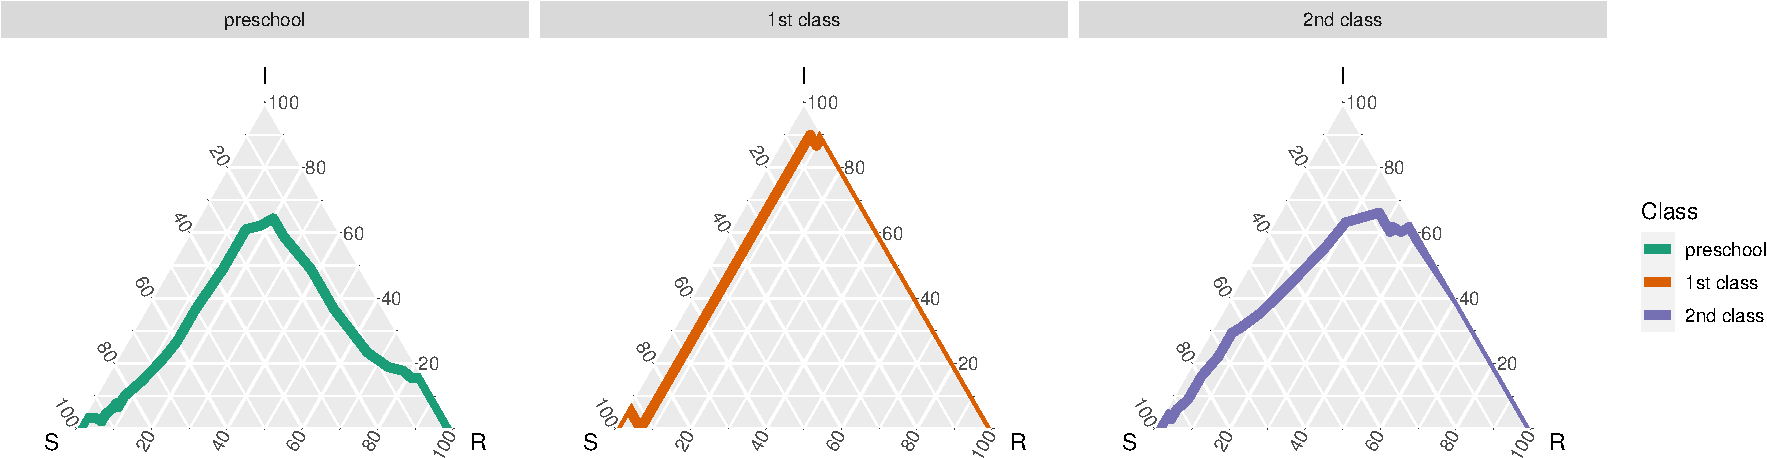
\includegraphics{Figs/unnamed-chunk-10-1} 

}

\caption{\label{fig:tern-class-data}Time invariant outbreak curves for the three class groups.  The pre-school class has a distinct peak of infection whereas the peak infection point for the other two classes are less well defined.}\label{fig:unnamed-chunk-10}
\end{figure}
\end{CodeChunk}

Along with multiple epidemic states, the function
\code{agents_to_aggregate} can also be extended to populations with
vital dynamics (e.g.~birth and death) and examples of this are shown in
the package vignette. In summary, \code{agents_to_aggregate()} is a
multi-purpose workhorse that may be leveraged to convert individual
level records into aggregate information that may be more useful for
some forms of epidemic modeling such as compartment modeling.

Up to this point, we have used \pkg{EpiCompare} in the context of
observed data. We also want to compare statistical models, and
\pkg{EpiCompare} aids in that process via a simple but dynamic
individual-level data generator, conversion tools for popular epidemic
model packages, and model assessments. We demonstrate an example here.

We first try to model the Hagelloch data with an SIR model (see Eq.
\ref{eq:sir}). In our vignette, we show how to fit a stochastic model
via maximum likelihood and simulate from the model with those best fit
parameters. Our function \code{simulate_agents()} generates individual
level data according to discrete multinomial draws, which depend on the
number of individuals in each state at the previous time step and a
matrix of transition probabilities. For example, the below code
generates 100 simulations of an outbreak of a diseease with one initial
infector in a population of \(n= 188\) individuals.

\begin{CodeChunk}
\begin{CodeInput}
R> trans_mat <- matrix(c("X0 * (1 - X1 * par1 / N)", "X0 * X1  * par1 / N", "0",
+                   "0", "X1 * (1 - par2)", "par2 * X1",
+                   "0", "0", "X2"), byrow = TRUE, nrow = 3)
\end{CodeInput}
\end{CodeChunk}

\begin{CodeChunk}
\begin{CodeInput}
R> set.seed(2020)
R> 
R> best_params <- c("beta" = .36, "gamma" = .13)
R> ## This is the SIR representation
R> 
R> rownames(trans_mat) <- c("S", "I", "R")
R> init_vals <- c(187, 1, 0)
R> par_vals <- c(par1 = best_params[1], par2 = best_params[2])
R> max_T <- 55
R> n_sims <- 100
R> 
R> agents <- simulate_agents(trans_mat,
+                        init_vals,
+                        par_vals,
+                        max_T,
+                        n_sims,
+                        verbose = FALSE)
\end{CodeInput}
\end{CodeChunk}

\begin{CodeChunk}
\begin{CodeInput}
R> agg_model <- agents %>% group_by(sim) %>%
+   agents_to_aggregate(states = c(I, R)) %>%
+   mutate(Type = "Simple SIR")
\end{CodeInput}
\end{CodeChunk}

The result of our simulation is the object \code{agents} which is a
18800 \(\times\) 5 which details the time of entry into the \(S\),
\(I\), and \(R\) states for a given simulation. Before we examine the
results of this simple SIR model, we will also examine another, more
sophisticated SIR model, this time from the package \pkg{EpiModel}.
Briefly, this model first fits a contact network to the set of
indivduals, where the class of the student is a covariate. The model
then simulates a SIR-epidemic on that network.

\begin{CodeChunk}
\begin{CodeInput}
R> library(EpiModel)
R> ## WARNING:  Will take a minute or two
R> 
R> set.seed(42)
R> nw <- network.initialize(n = 188, directed = FALSE)
R> nw <- set.vertex.attribute(nw, "group", rep(0:2, each = 90, 30, 68))
R> formation <- ~edges + nodematch("group") + concurrent
R> target.stats <- c(200, 300, 200)
R> coef.diss <- dissolution_coefs(dissolution = ~offset(edges),  duration = 5)
R> est1 <- netest(nw, formation, target.stats, coef.diss, edapprox = TRUE)
R> 
R> param <- param.net(inf.prob = 0.1, act.rate = 5, rec.rate = 0.1)
R> status.vector <- c(rep(0, 90), rep(0, 30), rep(0, 67), 1)
R> status.vector <- ifelse(status.vector == 1, "i", "s")
R> init <- init.net(status.vector = status.vector)
R> control <- control.net(type = "SIR", nsteps = 55,
+                        nsims = 100, epi.by = "group")
R> epimodel_sir <- netsim(est1, param, init, control)
\end{CodeInput}
\end{CodeChunk}

The output of this model is \code{epimodel_sir}, an object of class
netsim, which contains a plethora of modeling information. We provide
the function \code{fortify_aggregate()}, which can take objects from
specialized classes of modeling output and transform it into a
tidy-style data frame.

\begin{CodeChunk}
\begin{CodeInput}
R> fortified_net <- fortify_aggregate(epimodel_sir, 
+                                    states = c("s.num", "i.num", "r.num")) %>%
+   mutate(Type = "EpiModel SIR",
+          sim = as.numeric(gsub("sim", "", sim)))
\end{CodeInput}
\end{CodeChunk}

We can then analyze the results of the two models side by side as
time-invariant epidemic curves. The results are shown in Figure
\ref{fig:hag-simple-sir}, where a 90\% prediction band is estimated from
the delta ball method for each of the two models. For the Simple SIR
model, we see that the data generally covers the data fairly well but
clearly misses the second peak of infection. We also see that the
prediction band is very large, covering up a large area of the ternary
plot. On the other hand, for the \pkg{EpiModel} model, we see that the
prediction band covers the data quite well and takes up less area.

\begin{CodeChunk}
\begin{CodeInput}
R> both_models <- bind_rows(agg_model, fortified_net)
R> 
R> 
R> g <- ggplot() + geom_prediction_band(data = both_models %>% filter(t != 0),
+          aes(x = X0, y = X1, z = X2,
+               sim_group = sim, fill = Type),
+          alpha = .5,
+          conf_level = .90) 
\end{CodeInput}
\end{CodeChunk}

\begin{CodeChunk}
\begin{CodeInput}
R> g +   geom_path(data = both_models %>% filter(t !=0),
+             aes(x = X0, y = X1, z = X2, group = paste(Type, sim)),
+             alpha = .3, col = "gray40") + 
+     coord_tern() + theme_sir(base_size = 24) +
+   geom_point(data = hagelloch_sir,
+              aes(x = S, y = I, z =R), col = "black") +
+   labs(title = "Simple SIR model",
+        subtitle = "90% Prediction band and original data",
+        x = "S", y = "I", z = "R") +
+   scale_fill_manual(values = c("#006677", "#AA6600")) + 
+   facet_wrap(~Type) +
+   theme(legend.position = "bottom")
\end{CodeInput}
\begin{figure}[H]

{\centering 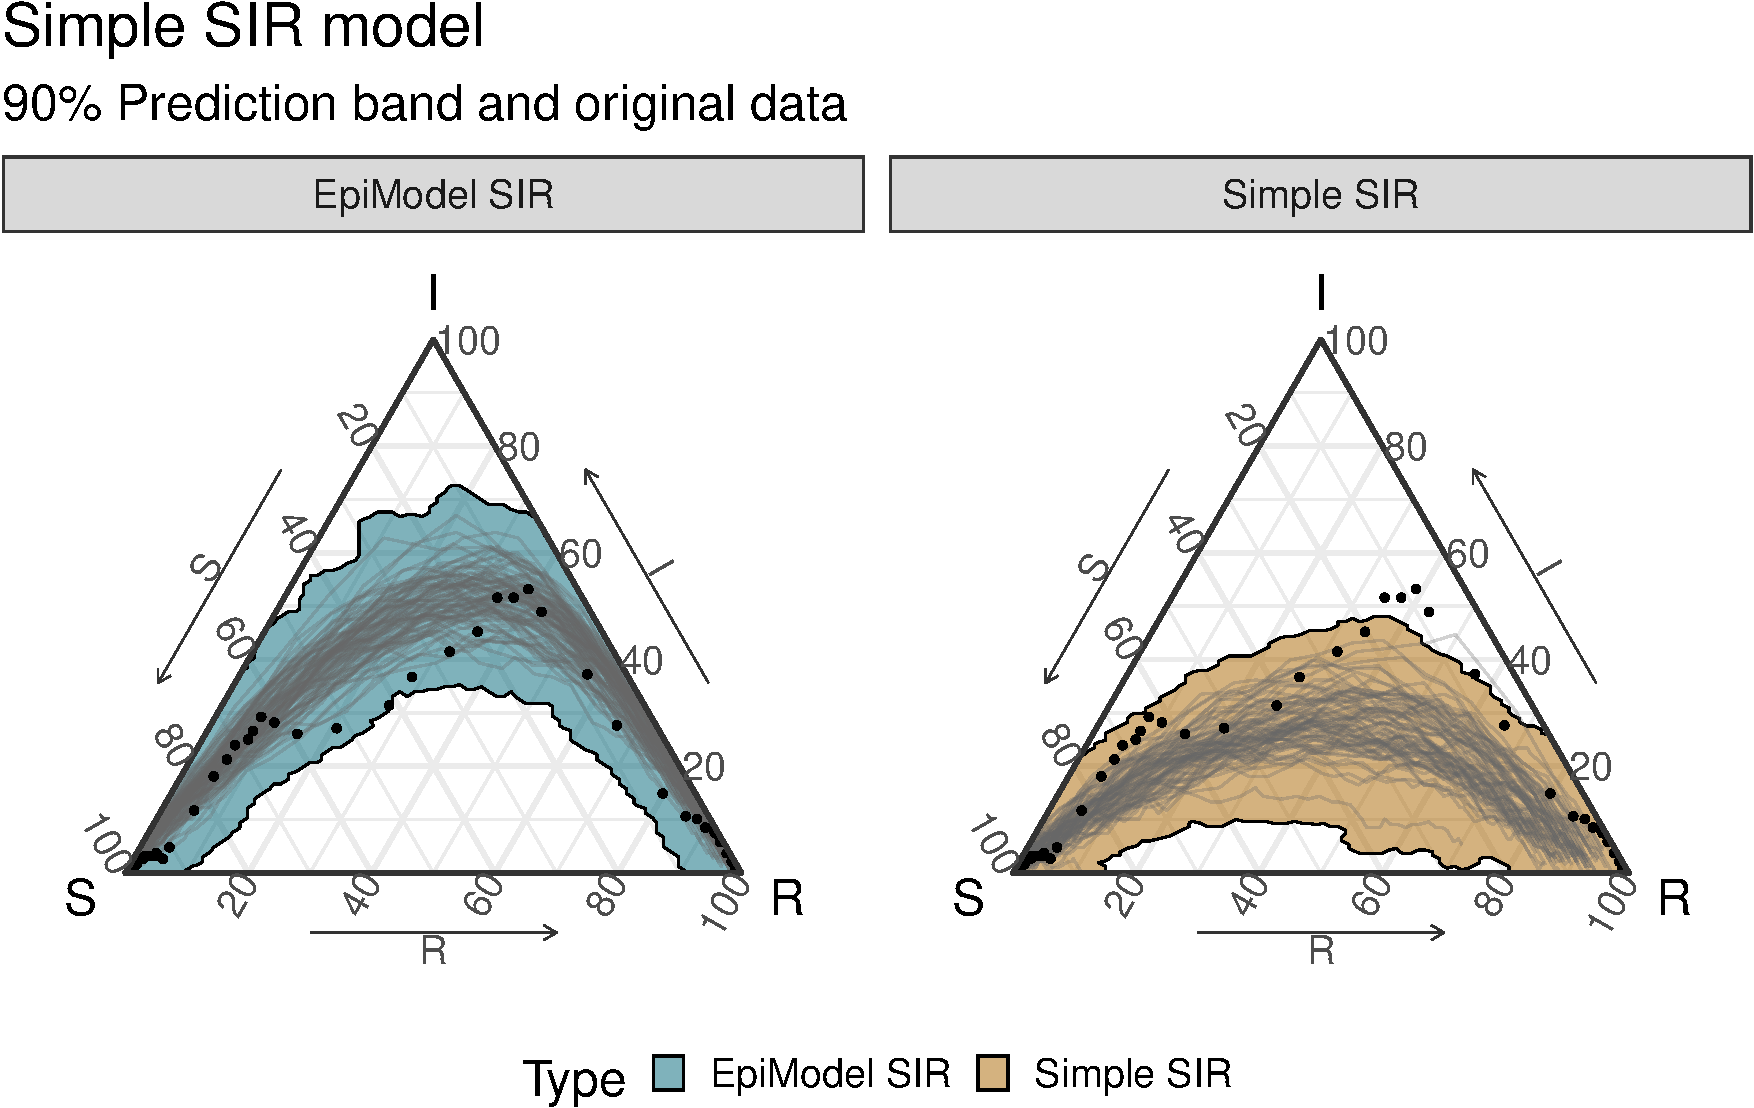
\includegraphics{Figs/unnamed-chunk-17-1} 

}

\caption{\label{fig:hag-simple-sir}  Original Hagelloch SIR data (black) along with 90\% prediction band and actual simulation paths from the Simple SIR and the EpiModel SIR models.}\label{fig:unnamed-chunk-17}
\end{figure}
\end{CodeChunk}

However, both models are not a good fit to the filamental path as
opposed to the individual points in \((S, I, R)\)-space. This can be
captures with the set of simulations both models predict, which all
generally have a single defined peak of infection whereas the data
certainly looks like it has two distinct peaks, likely caused by our
assumed super-spreader event. This observation is backed up by the below
analysis that demonstrates that the estimated psuedo-density of the
observed epidemic (relative to the simulations from either model) is
much less likely then \textbf{any} of the simulations (reported in Table
\ref{tab:hags-extreme}. In conclusion, \pkg{EpiCompare} makes it clear
that, at a glance, 1) the EpiModel network model is a better fit than
the Simple SIR model, and 2) the fit is only good at the individual
point level as opposed to the epidemic path level.

\begin{CodeChunk}
\begin{CodeInput}
R> #-- after cleaning up and combining --
R> all_together_df <- rbind(simple_sir,
+                          hagelloch_sir2)
\end{CodeInput}
\end{CodeChunk}

\begin{CodeChunk}
\begin{table}[!h]

\caption{\label{tab:cif-all-together-df}Top and bottom 2 rows of \tt{all\_together\_df}\text{, combining both simulated epidemics and the true epidemic.}}
\centering
\begin{tabular}[t]{lrrrrr}
\toprule
Type & sim & t & S & I & R\\
\midrule
Simple SIR & 1 & 0 & 188 & 0 & 0\\
Simple SIR & 1 & 1 & 187 & 1 & 0\\
true observation & 0 & 54 & 1 & 0 & 187\\
true observation & 0 & 55 & 1 & 0 & 187\\
\bottomrule
\end{tabular}
\end{table}

\end{CodeChunk}

\begin{CodeChunk}
\begin{CodeInput}
R> compression_df <- all_together_df %>% group_by(Type, sim) %>% 
+   filament_compression(data_columns = c("S","I","R"), 
+                        number_points = 20)
\end{CodeInput}
\end{CodeChunk}

\begin{CodeChunk}
\begin{CodeInput}
R> tdmat <- compression_df %>% 
+   dist_matrix_innersq_direction(
+     position = c(1:length(compression_df))[
+       names(compression_df) %in% c("S","I", "R")],
+     tdm_out = T)
R> 
R> simple_sir_true_obs_info <- tdmat %>% 
+   compare_new_to_rest_via_distance(
+     new_name_id = data.frame(Type = "true observation", sim = 0),
+     distance_func = distance_psuedo_density_function, 
+     sigma = "20%") 
\end{CodeInput}
\end{CodeChunk}

\begin{CodeChunk}
\begin{table}[!h]

\caption{\label{tab:hags-extreme}The extremeness of the true simulations based on comparing psuedo-density estimates between true vs simulated curves}
\centering
\begin{tabular}[t]{l>{\raggedleft\arraybackslash}p{6cm}>{\raggedleft\arraybackslash}p{6cm}}
\toprule
Type & simulations-based estimated psuedo-density & proportion of simulations with lower estimated psuedo-density\\
\midrule
Simple SIR & 0.0036733 & 0\\
EpiModel SIR & 0.0028813 & 0\\
\bottomrule
\end{tabular}
\end{table}

\end{CodeChunk}

\hypertarget{helpful-rmd-tricks}{%
\section{Helpful Rmd tricks}\label{helpful-rmd-tricks}}

\hypertarget{rmd-code-formatting-info}{%
\subsection{RMD Code formatting info}\label{rmd-code-formatting-info}}

This is the Section \ref{sec:intro}. This template demonstrates some of
the basic LaTeX that you need to know to create a JSS article.

In general, don't use Markdown, but use the more precise LaTeX commands
instead:

\begin{itemize}
\item
  \proglang{Java}
\item
  \pkg{plyr}
\end{itemize}

One exception is inline code, which can be written inside a pair of
backticks (i.e., using the Markdown syntax).

If you want to use LaTeX commands in headers, you need to provide a
\texttt{short-title} attribute. You can also provide a custom identifier
if necessary. See the header of Section \ref{r-code} for example.

\subsection[R code]{RMD \proglang{R} code}\label{r-code}

Can be inserted in regular R markdown blocks.

hags hags hags \cite{Neal2004}

\begin{CodeChunk}
\begin{CodeInput}
R> x <- 1:10
R> x
\end{CodeInput}
\begin{CodeOutput}
 [1]  1  2  3  4  5  6  7  8  9 10
\end{CodeOutput}
\end{CodeChunk}

\bibliography{EpiCompare.bib}


\end{document}

